%!TEX TS-program = xelatex
%!TEX encoding = UTF-8 Unicode
% Awesome CV LaTeX Template for CV/Resume
%
% This template has been downloaded from:
% https://github.com/posquit0/Awesome-CV
%
% Author:
% Claud D. Park <posquit0.bj@gmail.com>
% http://www.posquit0.com
%
% Template license:
% CC BY-SA 4.0 (https://creativecommons.org/licenses/by-sa/4.0/)
%


%-------------------------------------------------------------------------------
% CONFIGURATIONS
%-------------------------------------------------------------------------------
% A4 paper size by default, use 'letterpaper' for US letter
\documentclass[11pt, a4paper]{awesome-cv}

% Configure page margins with geometry
\geometry{left=1.4cm, top=.8cm, right=1.4cm, bottom=1.8cm, footskip=.5cm}

% Specify the location of the included fonts
\fontdir[fonts/]

% Color for highlights
% Awesome Colors: awesome-emerald, awesome-skyblue, awesome-red, awesome-pink, awesome-orange
%                 awesome-nephritis, awesome-concrete, awesome-darknight
\colorlet{awesome}{awesome-red}
% Uncomment if you would like to specify your own color
% \definecolor{awesome}{HTML}{CA63A8}

% Colors for text
% Uncomment if you would like to specify your own color
% \definecolor{darktext}{HTML}{414141}
% \definecolor{text}{HTML}{333333}
% \definecolor{graytext}{HTML}{5D5D5D}
% \definecolor{lighttext}{HTML}{999999}

% Set false if you don't want to highlight section with awesome color
\setbool{acvSectionColorHighlight}{true}

% If you would like to change the social information separator from a pipe (|) to something else
\renewcommand{\acvHeaderSocialSep}{\quad\textbar\quad}


%-------------------------------------------------------------------------------
%	PERSONAL INFORMATION
%	Comment any of the lines below if they are not required
%-------------------------------------------------------------------------------
% Available options: circle|rectangle,edge/noedge,left/right
% \photo{profile.png}
\name{Bingjie}{YAN} % (闫冰洁)
\position{Trustworthy Federated Learning{\enskip\cdotp\enskip}AI for Healthcare{\enskip\cdotp\enskip}Edge AI{\enskip\cdotp\enskip}Privacy-Preserving ML}
\address{Institute of Computing Technology, Chinese Academy of Sciences, \\ No.6 Kexueyuan South Road Zhongguancun, Haidian District, Beijing, China, 100190}

\mobile{(+86) 156-6667-6912}
\email{bj.yan@ieee.org}
\homepage{www.bj-yan.top}
\github{beiyuouo}
\googlescholar{DVsgN1sAAAAJ}{DVsgN1sAAAAJ}
% \orcid{0000-0002-8810-9689}{0000-0002-8810-9689}
\linkedin{bingjie-yan-ba968118b}
% \gitlab{gitlab-id}
% \stackoverflow{SO-id}{SO-name}
% \twitter{@twit}
% \skype{skype-id}
% \reddit{reddit-id}
% \extrainfo{extra informations}

\quote{"Keep the curiosity."}


%-------------------------------------------------------------------------------
\begin{document}

% Print the header with above personal informations
% Give optional argument to change alignment(C: center, L: left, R: right)
\makecvheader

% Print the footer with 3 arguments(<left>, <center>, <right>)
% Leave any of these blank if they are not needed
\makecvfooter
  {\today}
  {Bingjie YAN~~~·~~~Curriculum Vitae}
  {\thepage}


%-------------------------------------------------------------------------------
%	CV/RESUME CONTENT
%	Each section is imported separately, open each file in turn to modify content
%-------------------------------------------------------------------------------
%-------------------------------------------------------------------------------
%    SECTION TITLE
%-------------------------------------------------------------------------------
\cvsection{个人简述}


%-------------------------------------------------------------------------------
%    CONTENT
%-------------------------------------------------------------------------------
\begin{cvparagraph}

%---------------------------------------------------------
我是一名海南大学本科四年级在读学生,。
\end{cvparagraph}

%-------------------------------------------------------------------------------
%        SECTION TITLE
%-------------------------------------------------------------------------------
\cvsection{教育经历}


%-------------------------------------------------------------------------------
%        CONTENT
%-------------------------------------------------------------------------------
\begin{cventries}

%---------------------------------------------------------
\cventry
{硕士{\enskip\cdotp\enskip}计算机科学} % Degree
{中国科学院{\enskip\cdotp\enskip}计算技术研究所} % Institution
{中国·北京} % Location
{2022.09 - Exp. 2025.06} % Date(s)
{
    \begin{cvitems} % Description(s) bullet points
        \item {GPA: 87/100 (3.79/4)}
        % \item {荣获海南大学“三好学生”、“志愿服务标兵”、“最具创新精神和实践能力的大学生”、“优秀毕业生”荣誉称号}
        % \item {获得海南大学一等综合奖学金}
    \end{cvitems}
}

\cventry
{本科{\enskip\cdotp\enskip}软件工程大数据方向} % Degree
{海南大学{\enskip\cdotp\enskip}计算机与科学技术学院} % Institution
{中国·海南} % Location
{2018.09 - 2022.06} % Date(s)
{
    \begin{cvitems} % Description(s) bullet points
        \item {GPA: 89.69/100 (3.67/4),排名: 8/179(4\%),CET-4: 539,CET-6: 478}
        \item {荣获海南大学“三好学生”、“志愿服务标兵”、“最具创新精神和实践能力的大学生”、“优秀毕业生”等荣誉称号}
        \item {获得海南大学一等综合奖学金、二等综合奖学金}
    \end{cvitems}
}

%---------------------------------------------------------
\end{cventries}

%-------------------------------------------------------------------------------
%	SECTION TITLE
%-------------------------------------------------------------------------------
\cvsection{Selected Publications}

\cvparagraph{\textcolor{gray}{\textbf{Note:} Please refer to my \href{https://scholar.google.com/citations?hl=en&user=DVsgN1sAAAAJ}{Google Scholar} for the complete list. The total citation is over 240 and h-index is 4.}}

\begin{cvpublications}

%---------------------------------------------------------
\cvpublication
{KAMOFL: K-Asynchronous Multi-objective Federated Learning with Privacy, Efficiency, and Utility Trade-offs} % Title
{\textbf{B. Yan}, Y. Chen, Q. Chen, X. Jiang, Y. Kang and T. Zhang} % Authors
{IJCAI'24 (Under Review)} % Conference
{} % Date
{} % Description

%---------------------------------------------------------

\cvpublication
{FedEYE: A Scalable and Flexible End-to-end Federated Learning Platform for Ophthalmology} % Title
{\textbf{B. Yan}, D. Cao, X. Jiang, Y. Chen, W. Dai, et al} % Authors
{Cell Patterns (SCI, JCR-Q2, IF=6.5)} % Conference
{2024} % Date
{\href{https://www.cell.com/patterns/fulltext/S2666-3899(24)00019-9}{[PDF]}} % Description

%---------------------------------------------------------

\cvpublication
{AFL-CS: Asynchronous Federated Learning with Cosine Similarity-based Penalty Term and Aggregation} % Title
{\textbf{B. Yan}, X. Jiang, Y. Chen, C. Gao and X. Liu} % Authors
{IEEE ICPADS 2024 (CCF-C, Oral)} % Conference
{2023} % Date
{To be appeared.} % Description

%---------------------------------------------------------

\cvpublication
{Experiments of Federated Learning for COVID-19 Chest X-ray Images} % Title
{\textbf{B. Yan}, J. Wang, J. Cheng, et al} % Authors
{ICAIS 2021 (EI)} % Conference
{2021} % Date
{\textbf{Over 150 citations in Google Scholar.} \href{https://arxiv.org/abs/2007.05592}{[arXiv]} \href{https://link.springer.com/chapter/10.1007/978-3-030-78618-2_4}{[PDF]}
} % Description

%---------------------------------------------------------

\cvpublication
{FedCM: A Real-time Contribution Measurement Method for Participants in Federated Learning} % Title
{\textbf{B. Yan}, B. Liu, L. Wang, Y. Zhou, Z. Liang, M. Liu and C. Xu} % Authors
{IJCNN 2021 (CCF-C, Oral)} % Conference
{2021} % Date
{\href{https://arxiv.org/abs/2009.03510}{[arXiv]} \href{https://ieeexplore.ieee.org/abstract/document/9534451/}{[PDF]}} % Description

%---------------------------------------------------------

\cvpublication
{An Improved Method for the Fitting and Prediction of the Number of COVID-19 Confirmed Cases Based on LSTM} % Title
{\textbf{B. Yan}, J. Wang, Z. Zhen, et al} % Authors
{Computers, Materials \& Continua (SCI, JCR Q2)} % Conference
{2020} % Date
{\href{https://www.techscience.com/cmc/v64n3/39440/pdf}{[PDF]}} % Description

%---------------------------------------------------------


\end{cvpublications}

% %-------------------------------------------------------------------------------
% %	CONTENT
% %-------------------------------------------------------------------------------
% \begin{cventries}
% %---------------------------------------------------------


% % \cventry
% % {\underline{\textbf{B. Yan}}, Y. Chen, Q. Chen, X. Jiang, Y. Kang and T. Zhang} % Role
% % {KAMOFL: K-Asynchronous Multi-objective Federated Learning with Privacy, Efficiency, and Utility Trade-offs} % Title
% % {} % Location
% % {} % Date(s)
% % {
% % 	\textcolor{awesome-red}{IJCAI'24 (Under Review)}
% % }


% %---------------------------------------------------------
% \cventry
% {\underline{\textbf{B. Yan}}, D. Cao, X. Jiang, Y. Chen, W. Dai, et al.} % Role
% {FedEYE: A Scalable and Flexible End-to-end Federated Learning Platform for Ophthalmology} % Title
% {Cell Patterns (SCI, IF=6.5)} % Location
% {2024.02} % Date(s)
% {
% 	\textcolor{awesome-red}{\href{https://www.cell.com/patterns/fulltext/S2666-3899(24)00019-9}{[PDF]}}
% }

% %---------------------------------------------------------
% \cventry
% {\underline{\textbf{B. Yan}}, X. Jiang, Y. Chen, C. Gao and X. Liu} % Role
% {AFL-CS: Asynchronous Federated Learning with Cosine Similarity-based Penalty Term and Aggregation} % Title
% {IEEE ICPADS 2024 (CCF-C)} % Location
% {2023.12, Oral.} % Date(s)
% {
% 	\textcolor{awesome-red}{To be appeared.}
% }

% %---------------------------------------------------------
% \cventry
% {\underline{\textbf{B. Yan}}, J. Wang, J. Cheng, Y. Zhou, Y. Zhang, Y. Yang, L. Li, H. Zhao, C. Wang and B. Liu} % Role
% {Experiments of Federated Learning for COVID-19 Chest X-ray Images} % Title
% {ICAIS 2021 (EI)} % Location
% {2021.07} % Date(s)
% {	
% 	\textcolor{awesome-red}{\textbf{Over 150 citations in Google Scholar.~}}
% 	\textcolor{awesome-red}{\href{https://arxiv.org/abs/2007.05592}{[arXiv]}}
% }

% %---------------------------------------------------------
% \cventry
% {\underline{\textbf{B. Yan}}, B. Liu, L. Wang, Y. Zhou, Z. Liang, M. Liu and C. Xu} % Role
% {FedCM: A Real-time Contribution Measurement Method for Participants in Federated Learning} % Title
% {IJCNN 2021 (CCF-C)} % Location
% {2021.07, Oral.} % Date(s)
% {
% 	\textcolor{awesome-red}{\href{https://arxiv.org/abs/2009.03510}{[arXiv]}}
% }

% %---------------------------------------------------------
% \cventry
% {\underline{\textbf{B. Yan}}, J. Wang, Z. Zhen, X. Tang, Y. Zhou, G. Zheng, Q. Zou, Y. Lu, B. Liu, W. Tu and N. Xiong} % Role
% {An Improved Method for the Fitting and Prediction of the Number of COVID-19 Confirmed Cases Based on LSTM} % Title
% {Computers, Materials \& Continua (SCI, JCR Q2)} % Location
% {2020.05} % Date(s)
% {
% 	\textcolor{awesome-red}{\href{https://www.techscience.com/cmc/v64n3/39440/pdf}{[PDF]}}
% }

% 	%---------------------------------------------------------
% \end{cventries}

%-------------------------------------------------------------------------------
%	SECTION TITLE
%-------------------------------------------------------------------------------
\cvsection{Internships}


%-------------------------------------------------------------------------------
%	CONTENT
%-------------------------------------------------------------------------------

%\cvsubsection{Innovative business practices \& Competition}

\begin{cventries}
%---------------------------------------------------------
\cventry
{Object detection and medical application in Federated Learning} % Job title
{Research Intern @ FedML} % Organization
{Remote} % Location
{2022.06 - 2022.08} % Date(s)
{
    \begin{cvitems}
        \item {Research on object detection and medical application in Federated Learning with MLDevOps.} % TODO: more details
    \end{cvitems}
}
\end{cventries}

\cvsection{Project Experiences}

\begin{cventries}
%---------------------------------------------------------
\cventry
{Subject with Aier Eye Hospital} % Job titl
{Federated collaborative platform system for digital ophthalmology} % Organization
{Beijing, China} % Location
{2021.12 - 2023.06} % Date(s)
{
    \begin{cvitems}
        \item {Researching the design of the federated learning platform and system for ophthalmology}
        \item {Implementing asynchronous federated learning methods on the platform for medical applications.}
    \end{cvitems}
}

%---------------------------------------------------------
% \cventry
% {Research and demonstration of key technologies for federated collaborative modeling of cross-domain trusted fusion.} % Job title
% {Subject with China Unicom Research Institute} % Organization
% {Beijing, China} % Location
% {2022.10 - 2023.10} % Date(s)
% {
%     \begin{cvitems}
%         \item {Research on Federated Learning in digital ophthalmology.}
%     \end{cvitems}
% }

%---------------------------------------------------------
% \cventry
% {Host} % Job title
% {Smart Image: Medical Image Recognition System based on Federated Learning} % Organization
% {Hainan, China} % Location
% {2020.03 - PRESENT} % Date(s)
% {
% 	\begin{minipage}[b]{0.25\linewidth}
% 		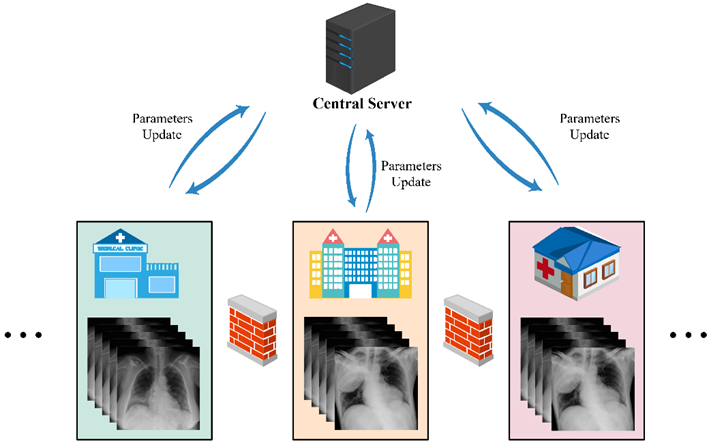
\includegraphics[height=8\baselineskip]{figure/fedcov.png}
% 	\end{minipage}
% 	\hfill
% 	\begin{minipage}[b]{0.7\linewidth}
% 		% 我们设计了一款基于联邦学习的医疗影像识别软件,可以在保护患者数据隐私的前提下进行多方联合。在数据方面,我们汇总了网上的多个公开数据集,并用Pydicom将dicom文件转换成图片形式用于模型识别。在模型方面,我们将包括ResNet、COVID-Net在内的4个模型进行模型融合,增强系统稳定性和泛化能力。同时,我们用GradCAM++对卷积层进行可视化,用于标记病灶位点,最后能够自动化生成医学报告。另外,在多方贡献衡量方面我们提出了FedCM贡献评估算法。
% 		We designed a medical image recognition software based on federated learning that allows for multi-party federation while protecting the privacy of patient data. In the aspect of data, we aggregate several published datasets on the Internet. In terms of models, we fused four models including ResNet and COVID-Net for model fusion to enhance system stability and generalization capability. We use GradCAM++ to visualize the convolutional layers for annotating lesion sites, and finally the software can generate medical reports automatically. In addition, we propose the FedCM contribution evaluation algorithm in the multiparty contribution measurement. \textcolor{awesome-red}{\href{https://github.com/beiyuouo/paddle-fl-gui}{[Code]}}
% 	\end{minipage}
% }

%---------------------------------------------------------
% \cventry
% {Participate} % Job title
% {5G Road Patrol Car} % Organization
% {Hainan, China} % Location
% {2020.05 - PRESENT} % Date(s)
% {
% 	\begin{minipage}[b]{0.25\linewidth}
% 		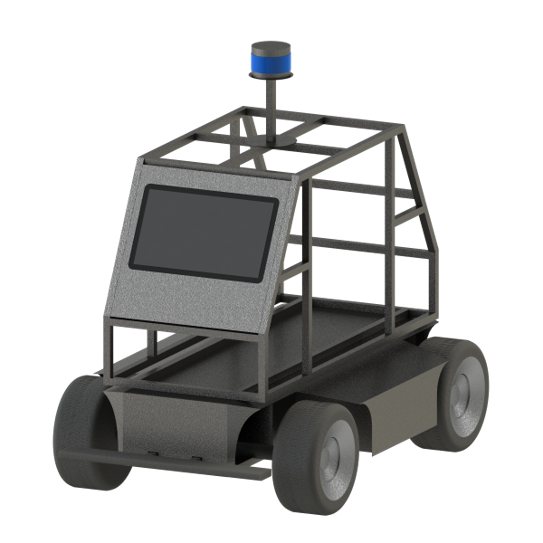
\includegraphics[height=8\baselineskip]{figure/car.png}
% 	\end{minipage}
% 	\hfill
% 	\begin{minipage}[b]{0.7\linewidth}
% 		% 我们设计了一款基于5G和多传感器融合用于城市巡逻的无人路检机器人,主要功能有基于多传感器融合的道路裂缝、坑洼等缺陷检测并进行云端上报,和违停检测。在建图和定位方面,我们基于LeGO-LOAM进行调整和改进。在道路检测方面,我们基于Yolov5训练了自己的模型,F1-score达到了0.68
% 		We designed an unmanned road inspection robot based on 5G and multi-sensor fusion for city patrol. The main functions are multi-sensor fusion-based detection of road cracks, potholes and other defects and reporting them to the cloud, and parking violation detection. For mapping and localization, we adapt and improve the algorithm based on LeGO-LOAM. For road detection, we have trained our own model based on Yolov5, and the F1-score reached 0.68.
% 	\end{minipage}
% }

%---------------------------------------------------------
% \cventry
% {Participate} % Job title
% {ROV technology-based underwater sightseeing robot.} % Organization
% {China} % Location
% {2020.05 - PRESENT} % Date(s)
% {
% 	This is a national student innovation and entrepreneurship project. We use underwater ROV for image collection and transmission. After defogging, we perform stitching of video frame sequences to achieve panoramic landscape viewing.
% }

%---------------------------------------------------------
%\end{cventries}

%\cvsubsection{Open Source Project}

%\begin{cventries}
%---------------------------------------------------------
%	\cventry
%	{Owner} % Job title
%	{FedMedical:PaddleFL-based Federated Learning Medical Image Recognition Software} % Organization
%	{\href{https://github.com/beiyuouo/paddle-fl-gui}{\color{awesome-red}{[GitHub link]}}} % Location
%	{2020.11 - PRESENT} % Date(s)
%	{
%		\begin{cvitems} % Description(s) of tasks/responsibilities
%			\item {Distributed Deployment and Federated Learning Simultaneous Training with PaddleFL Framework.}
%		\end{cvitems}
%	}

%---------------------------------------------------------
% \cventry
% {Owner} % Job title
% {Mid-air Draw: Gesture Recognition and Tracking based on YOLOv5} % Organization
% {Hainan, China} % Location
% {2020.09 - PRESENT} % Date(s)
% {
% 	We label the data ourselves and use YOLOv5 for gesture recognition and finger key point recognition. It is able to interact with PPT and other software to achieve the function of mid-air drawing. \textcolor{awesome-red}{\href{https://github.com/beiyuouo/mid-air-draw}{[Code]}} \textcolor{awesome-red}{\href{https://www.bilibili.com/video/BV15V411a7WB/}{[Video]}}
% }

	
%---------------------------------------------------------
\end{cventries}


%-------------------------------------------------------------------------------
%	SECTION TITLE
%-------------------------------------------------------------------------------
% \newpage
\cvsection{Open Source Contributions}

%-------------------------------------------------------------------------------
%	CONTENT
%-------------------------------------------------------------------------------
\begin{cventries}

%---------------------------------------------------------
\cvproject
{FedML-AI Community (contributor \& research intern)} % Project Title
{https://github.com/FedML-AI/FedML} % Project Link
{4k+} % Stars
{2022.06 - 2022.09} % Date(s)
{
\begin{cvitems} % Description(s) of tasks/responsibilities
\item {I enhance \href{https://github.com/FedML-AI/FedCV}{\textbf{FedCV}} with the popular object detection model (e.g. YOLOv5, YOLOv7, YOLOv8, etc.), deploy them to produce environment and provide technical support for the community.}
\item {I completely port the \href{https://github.com/owkin/FLamby}{\textbf{FLamby}} benchmark (contains 7 real-world federated datasets) to \href{https://open.fedml.ai/}{\textbf{FedML Open Platform}}.}
\end{cvitems}
} % Description


%---------------------------------------------------------

\cvproject
{hCaptcha-challenger (maintainer)} % Project Title
{https://github.com/QIN2DIM/hcaptcha-challenger} % Project Link
{1.3k+} % Stars
{2021.12 - 2023.10} % Date(s)
{
\begin{cvitems} % Description(s) of tasks/responsibilities
\item {We develop a robust AI-powered captcha solver utilizing Python and Selenium, effectively bypassing hCaptcha with an \textbf{accuracy exceeding 90\%}, and provide a user-friendly API for developers.}
\item {I utilize the CLIP model to achieve zero-shot captcha image classification and automatically labeling the captcha images via clustering. With the semenatic alignment ability of CLIP, the solver can achieve an open-set recognition.}
\item {I release the \href{https://github.com/CaptchaAgent/hcaptcha-model-factory}{\textbf{hcaptcha-model-factory~(\faStar 66)}} with a comprehensive workflow for community.}
\end{cvitems}
} % Description


%---------------------------------------------------------

\cvproject
{Awesome-FL (maintainer)} % Project Title
{https://github.com/youngfish42/Awesome-Federated-Learning-on-Graph-and-Tabular-Data}
{1.2k+} % Stars
{2023.06 - present} % Date(s)
{
\begin{cvitems} % Description(s) of tasks/responsibilities
\item {I actively contribute to the content, maintaine the repository, and keep up with the latest research in FL. }
\end{cvitems}
} % Description


%---------------------------------------------------------

\cvproject
{AI-Paper-Collector (maintainer)} % Project Title
{https://github.com/MLNLP-World/AI-Paper-Collector}
{1.1k+} % Stars
{2021.12 - 2022.12} % Date(s)
{
\begin{cvitems} % Description(s) of tasks/responsibilities
\item {We develop an automated paper collector from top AI conferences (NeurIPS, ICML, etc.) with web interface.}
\end{cvitems}
} % Description

%---------------------------------------------------------

\cvproject
{Personal Projects} % Project Title
{https://github.com/beiyuouo} % Project Link
{} % Stars
{\href{https://github.com/beiyuouo}{\textcolor{text}{\faGithub~\textbf{\underline{beiyuouo}}}} (150+ followers, 500+ stars)} % Date(s)
{
\begin{cvitems} % Description(s) of tasks/responsibilities
\item {\href{https://github.com/beiyuouo/arxiv-daily}{\textbf{arxiv-daily~(\faStar 77)}}: Automatically collect and push the latest arXiv papers to GitHub using GitHub Actions.}
\item {\href{https://github.com/beiyuouo/awesome-asynchronous-federated-learning}{\textbf{awesome-asynchronous-federated-learning~(\faStar 70)}}: A collection of papers about asynchronous federated learning.}
\item {\href{https://github.com/beiyuouo/mid-air-draw}{\textbf{mid-air-draw~(\faStar 17)}}: A simple hand-drawn and gesture recognition system using YOLOv5.}
\end{cvitems}
} % Description


%---------------------------------------------------------
\end{cventries}

%-------------------------------------------------------------------------------
%	SECTION TITLE
%-------------------------------------------------------------------------------
\cvsection{Selected Awards}


%-------------------------------------------------------------------------------
%	SUBSECTION TITLE
%-------------------------------------------------------------------------------
% \cvsubsection{International}


%-------------------------------------------------------------------------------
%	CONTENT
%-------------------------------------------------------------------------------
% \begin{cvhonors}

%---------------------------------------------------------
% \cvhonor
% {Silver} % Award
% {Asia-Pacific Informatics Olympiad, APIO} % Event
% {Beijing, China} % Location
% {2017} % Date(s)

%---------------------------------------------------------
% \end{cvhonors}


%-------------------------------------------------------------------------------
%	SUBSECTION TITLE
%-------------------------------------------------------------------------------
% \cvsubsection{International \& National}


%-------------------------------------------------------------------------------
%	CONTENT
%-------------------------------------------------------------------------------
\begin{cvhonors}

%---------------------------------------------------------
\cvhonor
{Silver} % Award
{(Intl.) Asia-Pacific Informatics Olympiad, APIO} % Event
{Beijing} % Location
{2017} % Date(s)

%---------------------------------------------------------
\cvhonor
{First Prize} % Award
{(Natl.) The 3rd Silk Road Robotics Innovations Competiton} % Event
{Xi'an} % Location
{2019} % Date(s)

%---------------------------------------------------------
\cvhonor
{Second Prize} % Award
{(Natl.) Contemporary Undergraduate Mathematical Contest in Modeling (CUMCM)} % Event China Collegiate Computing Contest
{Beijing} % Location
{2020} % Date(s)

%---------------------------------------------------------
\cvhonor
{Second Prize} % Award
{(Natl.) China Collegiate Computing Contest - Group Programming Ladder Tournament} % Event China Collegiate Computing Contest
{China} % Location
{2020} % Date(s)


%---------------------------------------------------------
\cvhonor
{Second Prize} % Award
{(Natl.) Chinese Collegiate Computing Competition} % Event
{Beijing} % Location
{2020} % Date(s)


%---------------------------------------------------------
\cvhonor
{Sliver \& Bronze} % Award
{(Natl.) The China Internation College Students' "Internet+" Innovation and Entrepreneurship Competition} % Event
{Beijing} % Location
{2023} % Date(s)

%---------------------------------------------------------
\cvhonor
{Third Prize} % Award
{(Natl.) China Collegiate Computing Contest - Artificial Intelligence Innovation Contest} % Event
{Hangzhou} % Location
{2020} % Date(s)


%---------------------------------------------------------
% \end{cvhonors}

% \cvsubsection{Provincial}


%-------------------------------------------------------------------------------
%	CONTENT
%-------------------------------------------------------------------------------
% \begin{cvhonors}

%---------------------------------------------------------
\cvhonor
{First Prize} % Award
{(Prov.) National Olympiad in Informatics in Provinces, NOIP} % Event
{Shandong} % Location
{2016} % Date(s)

%---------------------------------------------------------
\cvhonor
{First Prize} % Award
{(Prov.) China Collegiate Computing Contest - Group Programming Ladder Tournament} % Event
{Hainan} % Location
{2020} % Date(s)

%---------------------------------------------------------
\cvhonor
{Gold \& Sliver} % Award
{(Prov.) The 6th "Internet+" Innovation and Entrepreneurship Competition in Hainan} % Event
{Hainan} % Location
{2020} % Date(s)

%---------------------------------------------------------
\cvhonor
{First Prize} % Award
{(Prov.) Chinese Undergraduate Electronic Design Contest in Hainan} % Event
{Hainan} % Location
{2021} % Date(s)

%---------------------------------------------------------
\cvhonor
{Second Prize} % Award
{(Prov.) China Collegiate Computing Contest - Artificial Intelligence Innovation Contest} % Event
{South China} % Location
{2020} % Date(s)




%---------------------------------------------------------
% \cvhonor
% {Third Prize} % Award
% {The "Challenge Cup" College Students Extracurricular Science \& Technology Work Contest in Hainan.} % Event
% {Hainan} % Location
% {2021.05} % Date(s)

%---------------------------------------------------------
\end{cvhonors}

%-------------------------------------------------------------------------------
%	SECTION TITLE
%-------------------------------------------------------------------------------
% \cvsection{Leadership \& Membership}
\cvsection{SERVICES}
% \cvsection{Services}


%-------------------------------------------------------------------------------
%	CONTENT
%-------------------------------------------------------------------------------
\begin{cventries}
%---------------------------------------------------------
\cventryfour
{President, Student Membership} % Affiliation/role
{IEEE Hainan University Branch} % Organization/group
{Hainan, China} % Location
{2021.03 - 2022.06} % Date(s)


%---------------------------------------------------------
\cventryfour
{Vice President, Co-Founder} % Affiliation/role
{Association of Robotics and Artificial Intelligence, Hainan University} % Organization/group
{Hainan, China} % Location
{2020.07 - 2022.06} % Date(s)

%---------------------------------------------------------
% \cventry
% {Minister} % Affiliation/role
% {Youth Volunteer Association, Hainan University} % Organization/group
% {Hainan, China} % Location
% {2019.09 - 2020.07} % Date(s)
% {
% 	\begin{cvitems} % Description(s) of experience/contributions/knowledge
% 		\item {Participate in various volunteer activities.}
% 		\item {Enhance leadership and work distribution skills.}
% 	\end{cvitems}
% }

%---------------------------------------------------------
% \cventry
% {Vice President} % Affiliation/role
% {Cyberspace Security Association, Hainan University} % Organization/group
% {Hainan, China} % Location
% {2019.09 - 2020.07} % Date(s)
% {
% 	\begin{cvitems} % Description(s) of experience/contributions/knowledge
% 		\item {Learn about cyberspace security.}
% 		\item {Understand and carry out related work such as preparation of association activities.}
% 	\end{cvitems}
% }
%---------------------------------------------------------
\end{cventries}

\vspace{2mm}
%-------------------------------------------------------------------------------
%	SECTION TITLE
%-------------------------------------------------------------------------------
\cvsection{Skills \& Interests}


%-------------------------------------------------------------------------------
%	CONTENT
%-------------------------------------------------------------------------------
\begin{cvskills}
	
%---------------------------------------------------------
\cvskill
{Language} % Category
{Chinese(Native), English(Fluent, CET-6: 478, CET-4: 539, IELTS: working on!!)} % Skills

%---------------------------------------------------------
\cvskill
{Photography} % Category
{Enjoy the life and capture the moments :)} % Skills

%---------------------------------------------------------
%  \cvskill
%    {Programming languages} % Category
%    {Python, Java, C++} % Skills
%---------------------------------------------------------
	% \cvskill
	% {Machine Learning} % Category
	% {PyTorch, TensorFlow, OpenCV} % Skills
%---------------------------------------------------------
%	\cvskill
%	{Robotics} % Category
%	{ROS Melodic} % Skills
%---------------------------------------------------------
%   \cvskill
%     {Big data} % Category
%     {Hadoop, HBase, Hive, ZooKeeper, Storm, Kafka, Sqoop, Flume} % Skills
%---------------------------------------------------------
%	\cvskill
%	{Front-end} % Category
%	{Springboot, Mybatis, Flask} % Skills

%---------------------------------------------------------
\end{cvskills}

%%-------------------------------------------------------------------------------
%    SECTION TITLE
%-------------------------------------------------------------------------------
\cvsection{Presentation}


%-------------------------------------------------------------------------------
%    CONTENT
%-------------------------------------------------------------------------------
\begin{cventries}

%---------------------------------------------------------
  \cventry
    {Presenter for <DEFCON 20th : The way to go to Las Vegas>} % Role
    {6th CodeEngn (Reverse Engineering Conference)} % Event
    {Seoul, S.Korea} % Location
    {Jul. 2012} % Date(s)
    {
      \begin{cvitems} % Description(s)
        \item {Introduced CTF(Capture the Flag) hacking competition and advanced techniques and strategy for CTF}
      \end{cvitems}
    }

%---------------------------------------------------------
  \cventry
    {Presenter for <Metasploit 101>} % Role
    {6th Hacking Camp - S.Korea} % Event
    {S.Korea} % Location
    {Sep. 2012} % Date(s)
    {
      \begin{cvitems} % Description(s)
        \item {Introduced basic procedure for penetration testing and how to use Metasploit}
      \end{cvitems}
    }

%---------------------------------------------------------
\end{cventries}

%%-------------------------------------------------------------------------------
%	SECTION TITLE
%-------------------------------------------------------------------------------
\cvsection{Writing}


%-------------------------------------------------------------------------------
%	CONTENT
%-------------------------------------------------------------------------------
\begin{cventries}

%---------------------------------------------------------
  \cventry
    {Founder \& Writer} % Role
    {A Guide for Developers in Start-up} % Title
    {Facebook Page} % Location
    {Jan. 2015 - PRESENT} % Date(s)
    {
      \begin{cvitems} % Description(s)
        \item {Drafted daily news for developers in Korea about IT technologies, issues about start-up.}
      \end{cvitems}
    }

%---------------------------------------------------------
\end{cventries}

%%-------------------------------------------------------------------------------
%	SECTION TITLE
%-------------------------------------------------------------------------------
\cvsection{Program Committees}


%-------------------------------------------------------------------------------
%	CONTENT
%-------------------------------------------------------------------------------
\begin{cvhonors}

%---------------------------------------------------------
  \cvhonor
    {Problem Writer} % Position
    {2016 CODEGATE Hacking Competition World Final} % Committee
    {S.Korea} % Location
    {2016} % Date(s)

%---------------------------------------------------------
  \cvhonor
    {Organizer \& Co-director} % Position
    {1st POSTECH Hackathon} % Committee
    {S.Korea} % Location
    {2013} % Date(s)

%---------------------------------------------------------
  \cvhonor
    {Staff} % Position
    {7th Hacking Camp} % Committee
    {S.Korea} % Location
    {2012} % Date(s)

%---------------------------------------------------------
  \cvhonor
    {Problem Writer} % Position
    {1st Hoseo University Teenager Hacking Competition} % Committee
    {S.Korea} % Location
    {2012} % Date(s)

%---------------------------------------------------------
  \cvhonor
    {Staff \& Problem Writer} % Position
    {JFF(Just for Fun) Hacking Competition} % Committee
    {S.Korea} % Location
    {2012} % Date(s)

%---------------------------------------------------------
\end{cvhonors}



%-------------------------------------------------------------------------------
\end{document}
